\chapter{Machine Learning}

In this chapter a few classification models are evaluated for the feature extraction processes described in the preceding chapter. Two linear and six non linear models for supervised learning are compared using leave-one-out (\gls{loo}) cross validation on the acquired data. The workflow for all models apart from the last one follows the chart in figure \ref{fig:flow} where both training and test data use extracted features for classification.

% Define block styles
\tikzstyle{decision} = [diamond, draw, fill=blue!20, 
    text width=7.5em, text badly centered, inner sep=0pt]
\tikzstyle{block} = [rectangle, draw, fill=blue!20, 
    text width=7em, text centered, rounded corners, minimum height=4em]
\tikzstyle{line} = [draw, -latex']
\tikzstyle{cloud} = [draw, ellipse,fill=red!20, node distance=3cm,
    minimum height=4em]
\tikzstyle{blockgreen} = [rectangle, draw, fill=green!20, 
    text width=7em, text centered, rounded corners, minimum height=4em]
\tikzstyle{blockbrown} = [rectangle, draw, fill=brown!20, 
    text width=7em, text centered, rounded corners, minimum height=4em]

\begin{figure}
\centering
\begin{tikzpicture}[node distance = 3cm, auto]
	% Place nodes
	\node [blockbrown] (obtained) {Obtained data};
	\node [blockgreen, below left of=obtained] (training) {Training data};
	\node [block, below right of=obtained] (test) {Test data};
	\node [blockgreen, below of=training, node distance=2.2cm] (train pre) {Preprocess and extract features};
	\node [block, below of=test, node distance=2.2cm] (test pre) {Preprocess and extract features};
	\node [blockgreen, below right of=train pre] (est) {Estimate $\mathbf{\mu}_f$, $\mathbf{\sigma}_f$};
	\node [blockgreen, below left of=est] (scale train) {Scale to ZMUV};
	\node [block, below right of=est] (scale test) {Scale to ZMUV};
	\node [cloud, below right of=scale train] (train model) {Train model};
	\node [decision, below of=train model] (classify) {Classification};
	\node [block, below of=classify] (post) {Postprocessing};
	\node [block, below of=post, node distance=2.2cm] (output) {Model output};
	% Draw lines
	\path [line] (obtained) -| (training);
	\path [line] (obtained) -| (test);
	\path [line] (training) -- (train pre);
	\path [line] (test) -- (test pre);
	\path [line, dashed] (train pre) -| (est);
	\path [line,dashed] (est) -- (scale train);
	\path [line,dashed] (est) -- (scale test);
	\path [line] (test pre) -- (scale test);
	\path [line] (train pre) -- (scale train);
	\path [line] (scale train) |- (train model);
	\path [line] (train model) -- (classify);
	\path [line] (scale test) |- (classify);
	\path [line] (classify) -- (post);
	\path [line] (post) -- (output);
\end{tikzpicture}
\caption{Flowchart of classification scheme. Both training- and test data is preprocessed and scaled so that each feature has zero mean, unit variance. The training data is used to obtain model weighths, which become inputs to the classifier. Using these weights, predictions are made on the test data. These predictions then go through a postprocessing which results in the final output.}
\label{fig:flow}
\end{figure}




\section{Linear Models}

Linear classifiers performs a classification decision based on the value of a linear combination of input data \citep{santos_2018}. In the binary case this corresponds to dividing the dataset with a single hyperplane splitting data into two categories. New test data is then mapped into the same space and predicted to belong to a category based on which side of the hyperplane they fall. In this work, two linear models are considered: linear discriminant analysis (\gls{lda}) and a support vector machine (\gls{svm}) with a linear kernel. 
 
% Maybe throw in an equation here somewhere?

% This source doesn't really say this imo.
%Linear models are widely used in practice as they are general, and can therefore be used in many cases \citep{shalev-shwartz_ben-david_2016}.  Furthermore, they are relatively easy to understand, in contrast to more complex models such as neural networks. Despite this, they can often produce a decent accuracy with a low complexity.


\subsection{Linear Discriminant Analysis}

Linear discriminant analysis is an algorithm commonly used for dimensionality reduction \citep{raschka_2014}, but can also be used for classification purposes. \gls{lda} projects given data onto a subspace in a manner that separates the classes as much as possible. 

\gls{lda} bears many similarities to \gls{pca} in that it is based on finding eigenvectors with the largest corresponding eigenvalues, with the key difference that \gls{pca} disregards class labels whereas \gls{lda} does not. For further reading about \gls{lda}, we refer to \citep{raschka_2014}.


% Reducing the dimensionality of data is a good way of both lowering computational costs and avoiding overfitting as well as other phenomena that stem from a high-dimensional data. 

\subsection{Support Vector Machines}

Support vector machines are one of the most popular models when it comes to supervised learning. The most simple \gls{svm} uses what is called a linear kernel, and generates a linear hyperplane that separates two sets of labeled data similarly to \gls{lda}. Unlike \gls{lda} however, \gls{svm} is not an eigen-based method, making \gls{svm} less prone to outliers. Finding a good hyperplane is often an ambiguous task, so to find what the \gls{svm} regards as the best hyperplane it seeks parameters that maximize the distance between the hyperplane and the sample points closest to it known as support vectors \citep{boswell_2002}. 

% Commented out because we don't really use this
%Even if support vector machines are linear models, they are not limited to work only on linearly separable data. There are ways to use them in a non-linear fashion by utilizing different kinds of kernels. In principle, the data is first transformed into a higher dimensional space, including non-linear terms. In this new space, the \gls{svm} is used just as before. This makes the \gls{svm} a powerful tool even in non-linear problems \citep{boswell_2002}.

\section{Non-linear Models}
In many cases data cannot be satisfactorily separated by a linear classifier. In the binary case this means that the two classes in the dataset cannot be properly split by any one hyperplane. For such data non-linear algorithms may perform better. In this work, four different non-linear classification methods are tested: random forest (\gls{rf}), logistic regression (\gls{lr}), as well as two types of artificial neural network (\gls{ann}) classifiers. 

%Hence, if a linear model were to be trained on data that is not linearly separable, one would expect to notice a poor result in comparison to the result of a non-linear model. 

%The non-linear models considered in this work are random forest, logistic regression, as well as two kinds of neural networks.

\subsection{Random Forest}
Random forest (\gls{rf}) is an ensamble learning method that can be used for both regression- and classification problems. The name stems from that the method is based on several \textit{decision trees}, which are initiated randomly. A decision tree is a classifier per se, and is structured as a sequence of simple questions. These questions typically ask if a value is equal to or greater/smaller than some set value. The answers to these questions form a path in the decision tree, leading to an end node which corresponds to the prediction.

Random forest segments the training data into $n$ parts, and induces a decision tree from each group of data. Thus there are $n$ predictors that work independently, and by selecting the most common prediction, random forest yields a robust result with little risks of overfitting due to the combined results of many trees. On top of that it offers a very high accuracy in a wide variety of applications, while still maintaining an intuitive model structure that allows us to, for instance, estimate which features are important \citep{breiman_2002}. In Google's \emph{Project Soli}, random forests were used for millimeter-wave radar gesture recognition with impressive results \citep{lien_gillian_karagozler_amihood_schwesig_olson_raja_poupyrev_2016}. 

\subsection{Logistic Regression}
Logistic regression (\gls{lr}) is simlar to ordinary linear regression in that both methods aim to estimate parameters that describe the relationship between input and output variables. In linear regression, the parameters $\{b_i\}_{i=0}^n$ are modeled using the input variables $\{X_i\}_{i=1}^n$ and output variables $Y$ through
\begin{equation}
	Y= b_0+\sum_{i=1}^n b_iX_i.
\end{equation}

The key difference between the two is that \gls{lr} outputs continuous values without any boundaries, whereas logistic regression outputs a value in the open interval (0,1).  To achieve this, \gls{lr} transforms the result of the linear regression using the sigmoid function, defined as $f(z)=\frac{1}{1+e^{-z}}$. With this function, \gls{lr} instead maps the input variables to
\begin{equation}
	Y= \frac{1}{1+\exp(-(b_0 + \sum_{i=1}^n b_iX_i))}.
\end{equation}

This value is interpreted as a prediction confidence and can be used for making a decision in a binary classification.

Another major difference between linear and logistic regression is the choice of cost function. \gls{lr} commonly uses a cost function known as Cross-Entropy or Log Loss as opposed to Mean Squared Error, which is used for linear regression. For further details about \gls{lr}, including its cost function, we refer to \citep{a_smola_svn_vishwanathan_2010}.

\subsection{Artificial Neural Networks}
Artificial neural networks constitute a class of nonlinear models designed to mimic biological neural systems \citep{rojas_1996}. \gls{ann}s consist of multiple layers of neurons, or nodes. The networks are structured with an input layer followed by one or more hidden layers and one output layer \citep{logan_2017}. Figure \ref{fig:ann} illustrates a simple network which takes a feature vector $\mathbf{x}^{(0)}=[x_1^{(0)}\text{ }  x_2^{(0)}]^{T}$ as input. By multiplying the feature vector with a set of weights $\mathbf{w}^{(1)}$ the features are propagated through the network, generating a set of new node values. In the network in figure \ref{fig:ann} the output from the input layer, forwarded to the hidden layer, becomes
%\rowcolors{2}{white}{white}
\begin{equation}
	\mathbf{x}^{(1)}=\begin{bmatrix}x_1^{(1)} \\ x_2^{(1)} \\ x_3^{(1)} \end{bmatrix} = 
	\begin{bmatrix} w_{11}^{(1)} & w_{21}^{(1)} \\ w_{12}^{(1)} & w_{22}^{(1)} \\ w_{13}^{(1)} & w_{23}^{(1)}\end{bmatrix}\cdot \begin{bmatrix}x_1^{(0)} \\ x_2^{(0)}\end{bmatrix}.
\end{equation}

Here we omit the bias term in the hidden layer labeled "1". A bias term is an external, constant input to a layer, with trainable weights assigned to it. The bias term is independent of inputs from the previous layer and increases the flexibiliy of a model, thus making it more capable of fitting to the training data \citep{kohl_2010}. The bias term is represented by the top node within the hidden layer in figure \ref{fig:ann}. 

When the nodes in the hidden layer receives the propagated values they may range anywhere from negative to positive infinity. Using an \textit{activation function} $f$, the node transforms the input to a more suitable format in terms of whether the node should be "active" or not (or in biological terms, whether the neuron should fire) \citep{kriesel_2007}. The function $f$ also introduces non-linearity in the model, making \gls{ann}s capable of solving non-linear problems. 
% Wait with this to later?
%The choice of activation function is one of many things to consider when specifying hyperparameters.

Next, the output from the activation function is propagated with a new set of weights $\mathbf{w}^{(2)}$
\begin{equation}
	\mathbf{x}^{(2)}=\begin{bmatrix}x_1^{(2)} \\ x_2^{(2)} \end{bmatrix} = 
	\begin{bmatrix} w_{11}^{(2)} & w_{21}^{(2)} & w_{31}^{(2)} \\ w_{12}^{(2)} & w_{22}^{(2)} & w_{32}^{(2)} \end{bmatrix}\cdot \begin{bmatrix}f(x_1^{(1)}) \\ f(x_2^{(1)}) \\ f(x_3^{(1)}) \end{bmatrix}.
\end{equation}

The propagated values in $\mathbf{x}^2$ are the inputs to the output layer which after application of the activation function produces the output that is interpreted as a classification prediction. The model weights $\mathbf{w}^{(i)}$ of a neural network are commonly set through \textit{backpropagation} during the model training phase. For details about backpropagation, we refer to chapter 7 in \citep{rojas_1996}.

By introducing more than one hidden layer, the \gls{ann} can be called a deep neural network (\gls{dnn}). With the increased number of hidden layers, \gls{dnn}s are capable of extracting more complex patterns from data such as for image recognition \citep{szegedy_liu_jia_sermanet_reed_anguelov_erhan_vanhoucke_rabinovich_2018} or modeling of speech \citep{hinton_deng_yu_dahl_mohamed_jaitly_senior_vanhoucke_nguyen_sainath_2012}. Since we in the preceding chapter performed feature extraction the it should however not be necessary in this case to have more hidden layers than two, since useful features are already readily available.
%\gls{dnn}s in various forms have gained immense popularity over the past two decades achieving considerable success within a wide spectrum of applications, such as in image recognition and acoustic modeling of speech .v

\begin{figure}[h]
	\centering
	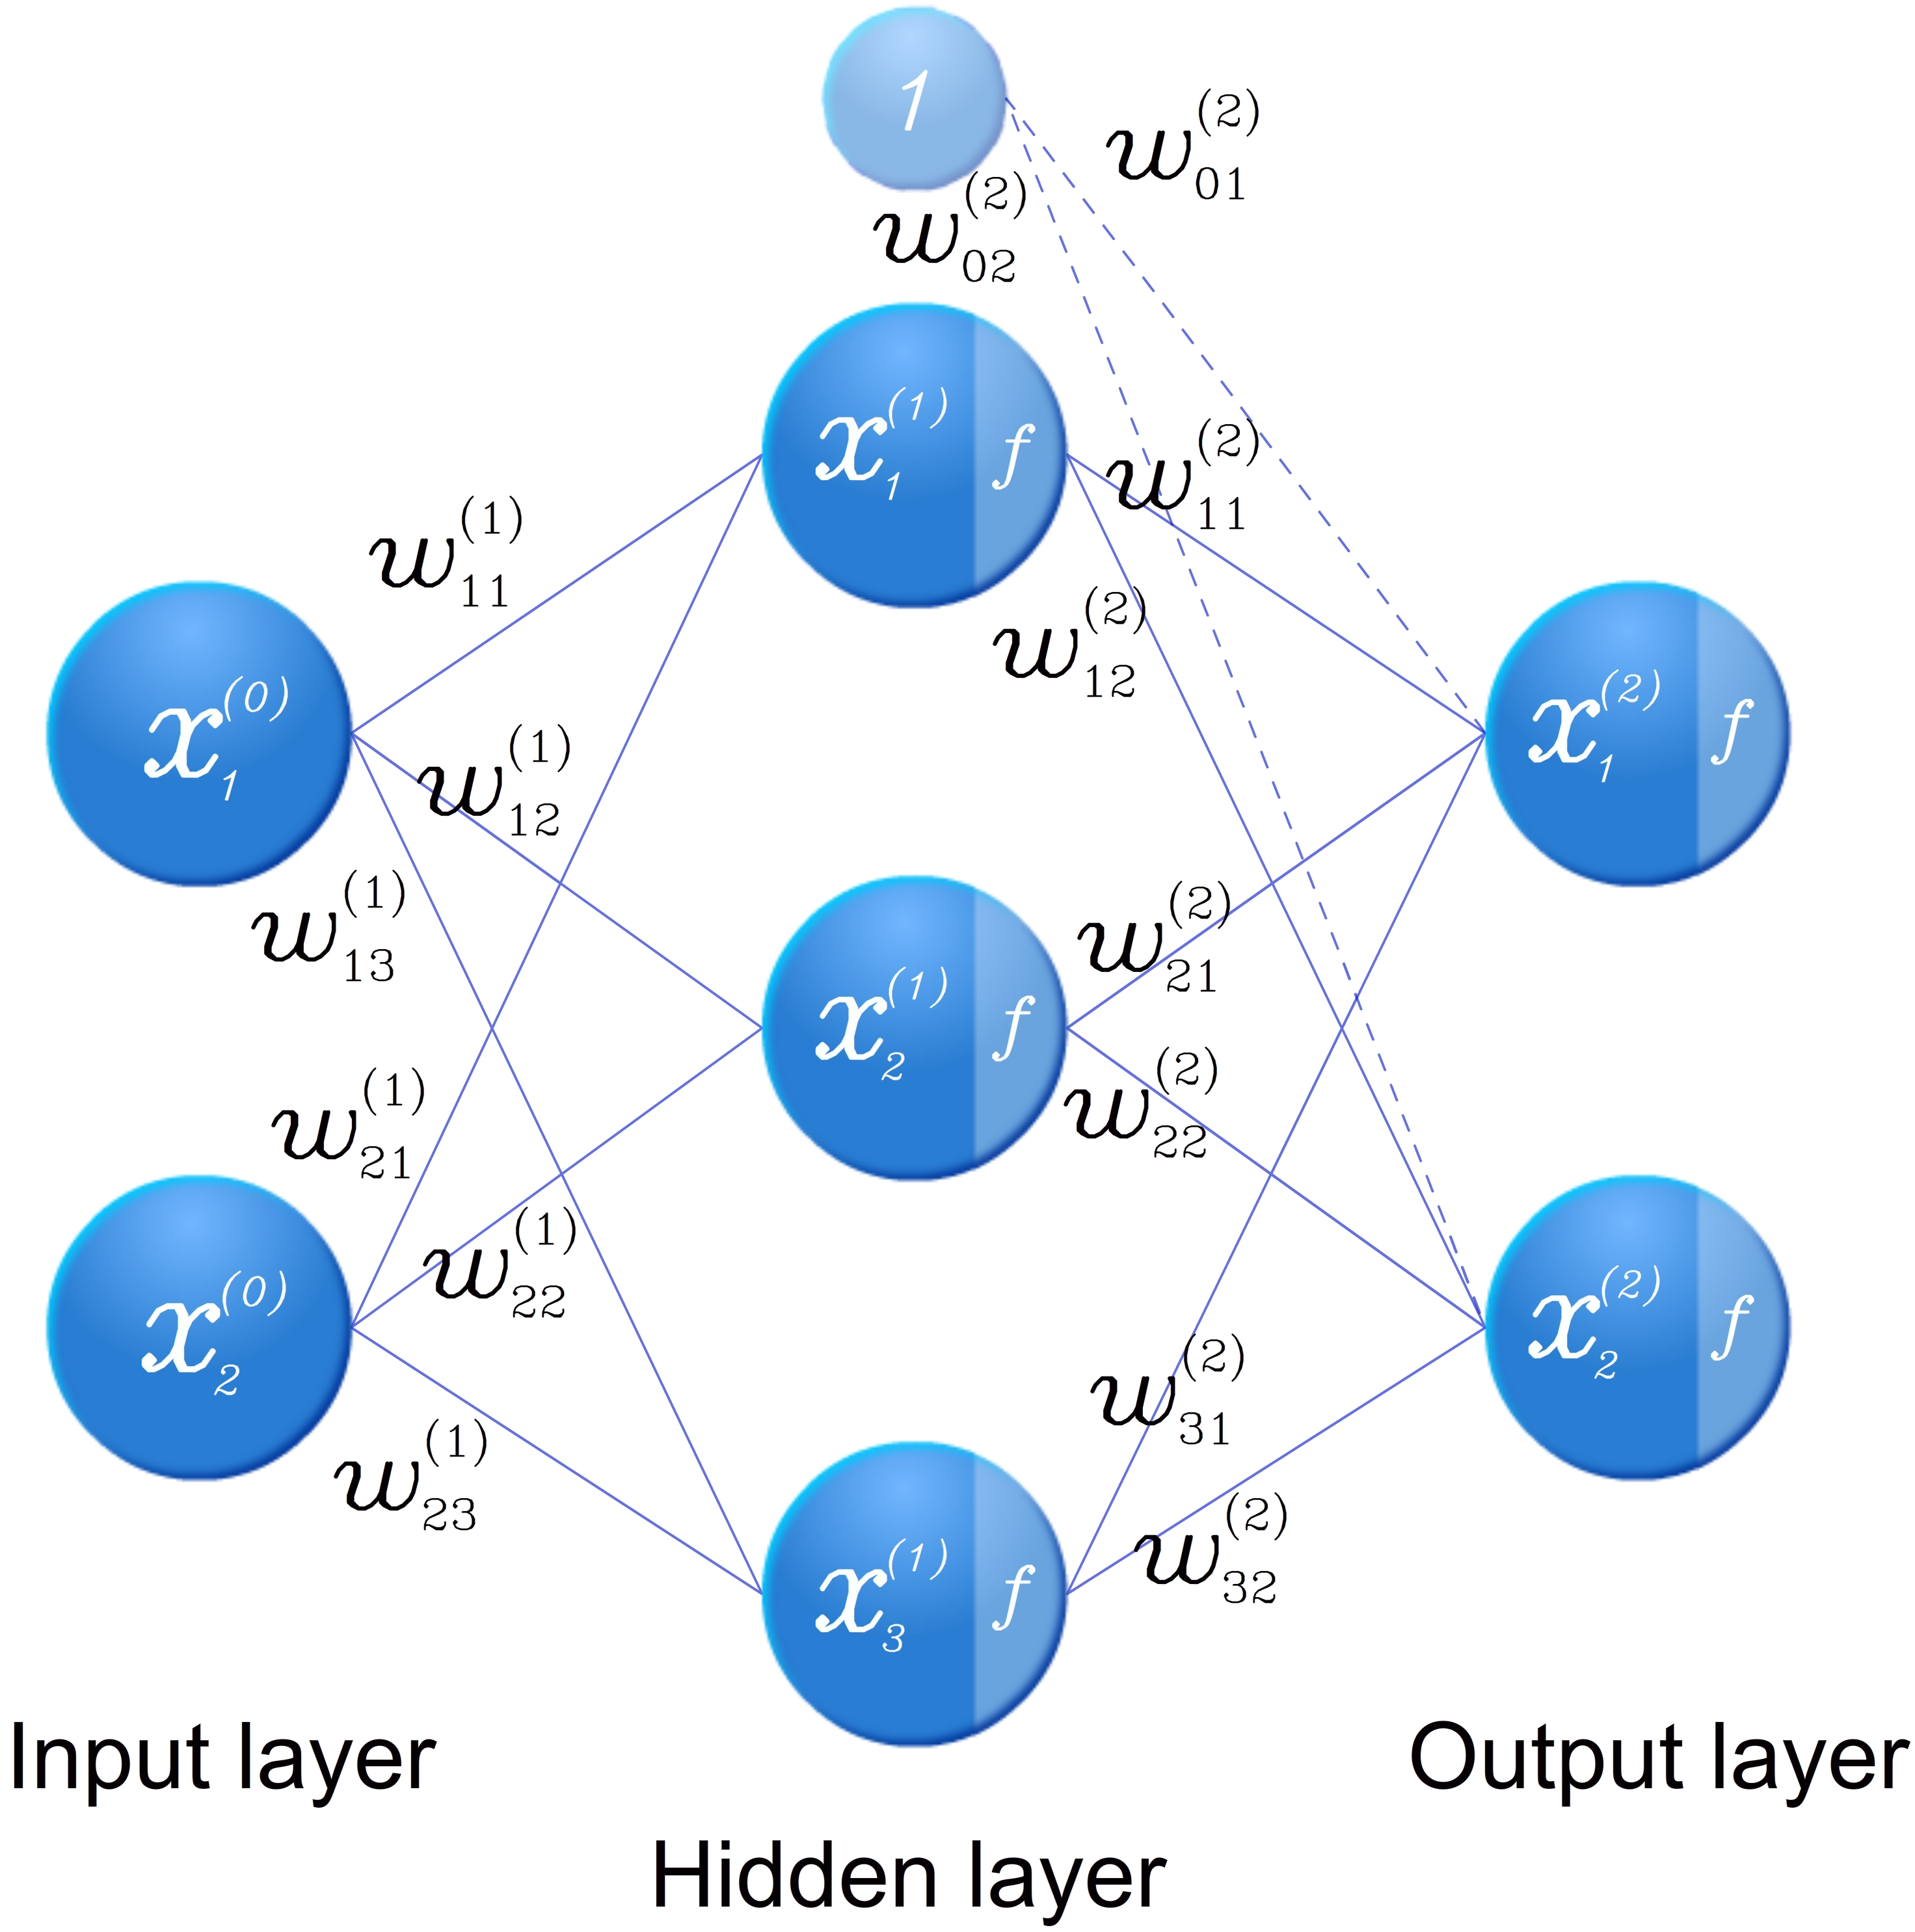
\includegraphics[scale=0.3]{figs_temp/network_graph.jpg}
	\caption{A simple neural network with 2 inputs, 2 outputs, and one hidden layer. The top node in the hidden layer is a bias term which can be added for increased flexibility during training.}
	\label{fig:ann}
\end{figure}

\subsubsection{Hyperparameters of Neural Networks}

The sizes of input and output layers are determined by the classification problem, but the internal structure of a \gls{dnn} classifier can be structured freely. The number of hidden layers and the number of nodes therein should be selected with care, as increasing the model size rapidly increases the computational complexity and the number of trainable parameters. When it comes to reducing overfitting \emph{dropout} is a method commonly utilized in nerual networks. By randomly disabling some of the hidden layer nodes during the training phase the model is forced to become more general not relying on any specific set of nodes for accomplishing its target. A node $n$ in layer $k$ is disabled by setting the weights $w^{(k)}_{nj}$ to 0, where $j$ ranges from 1 to the number of nodes in the sequent layer. For any node in a layer that features dropout, the \textit{dropout rate} specifies the probability that the node will be disabled.

While the above parameters relate to the architecture of the network, there are additional parameters that are related to the training process. The \emph{batch size} specifies how many samples are propagated through the network inbetween each update of the model weights. A small batch size has the benefit of requiring little memory and converging quickly, but at the same time impairs the gradient estimate \citep{brownlee_2017}. With a larger batch size the gradient is more accurately estimated but convergencence is slower. 

If the total number of samples is $m$, and the batch size is $b$, there will be $m/b$ forward and backward propagations, and equally many model weight updates. Each batch is only propagated once, but to extend the model training process even further, we can specify number of \emph{epochs}. This hyperparameter determines how many times each batch will be fed through the model. Often, one epoch is not enough for the weights to fully converge \citep{kriesel_2007}. Increasing the number of epochs naturally increases the training time and on top of that too many epochs puts the model at risk of overfitting.
% "too many epochs puts the model at risk of overfitting." is this really true? If so from what source. 

\begin{figure}[h]
	\centering
	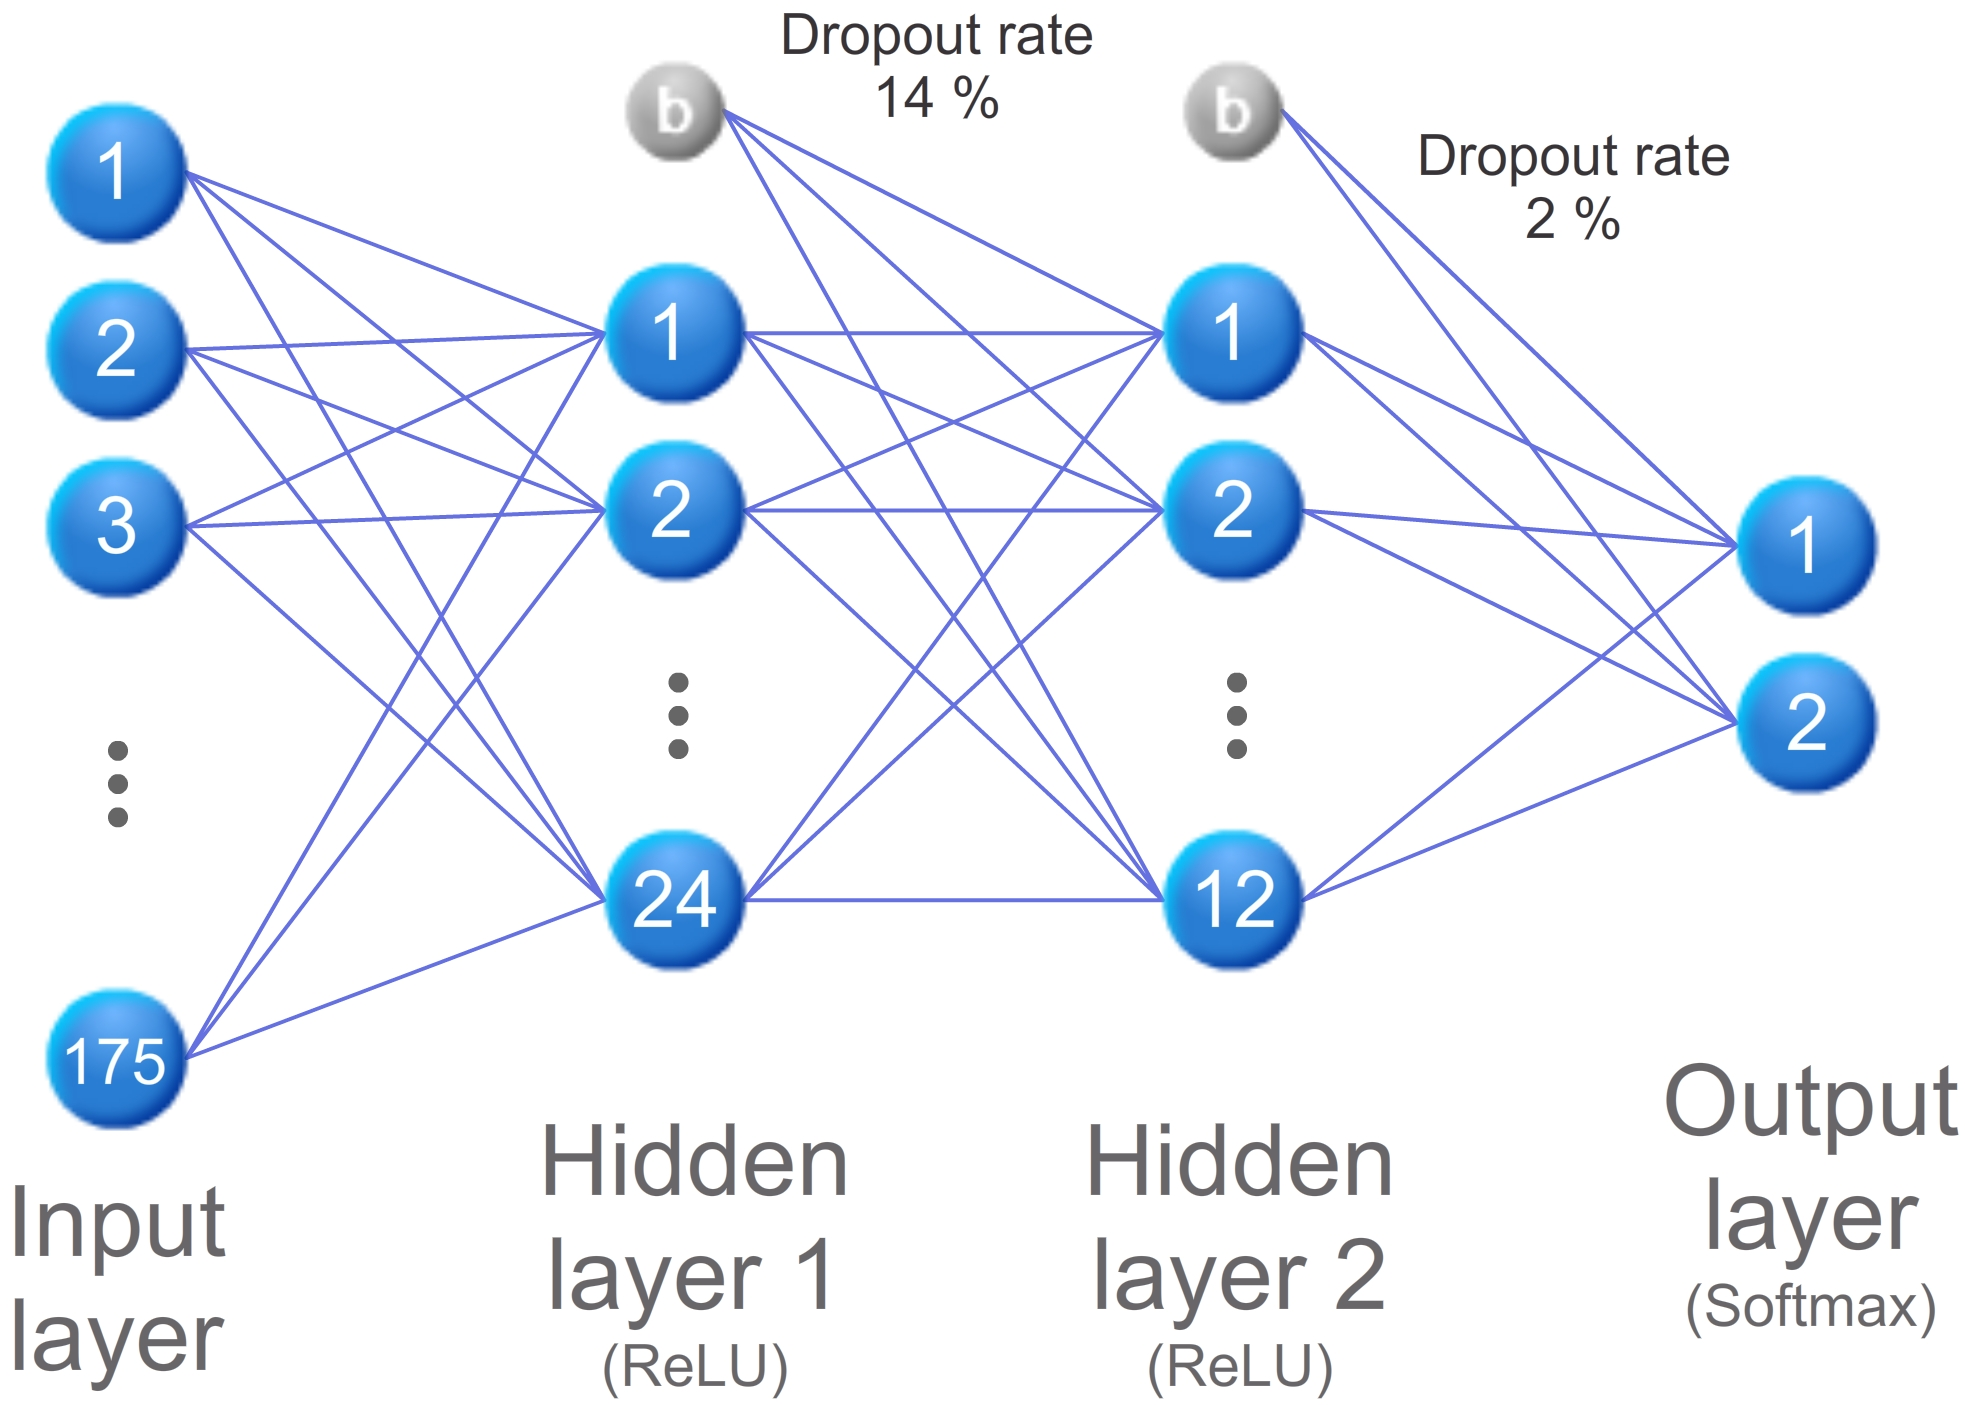
\includegraphics[scale=0.5]{figs_temp/optimized_network_graph.jpg}
	\caption{Using Hyperas, a network with two hidden layers was optimized in terms of number of nodes, dropout rate and activation function among other things. The resulting network has 25 and 13 nodes - including bias terms - in the hidden layers, and dropout rates of 14 and 2 percent, respectively. The hidden layers were assigned the ReLU activation function.}
	\label{fig:opt_net}
\end{figure}

The hyperparameters of the \gls{dnn} model was optimized using the free optimization tool Hyperas (available on GitHub at \url{https://github.com/maxpumperla/hyperas}). Hyperas selected the number of nodes, the dropout rates, the batch size and the optimization algorithm (from the three options of RMSprop, Adam and Stochastic Gradient Descent natively available in Keras). 

With the selections made by Hyperas, the network in figure \ref{fig:opt_net} is obtained. The two hidden layers have 24 and 12 nodes with dropout rates of 14 and 2 percent respectively. Both layers have the activation function $f(x)=\textrm{max}(0,x)$ often referred to as rectified linear unit (ReLU) and the output layer has a \textit{softmax} activation function. Furthermore the batch size in the learning phase is 32, and the number of epochs is set to 20. Finally, the optimization algorithm prefered by Hyperas is RMSprop.

\subsection{Convolutional Neural Network with Long Short Term Memory}
In previous models normalized data went through a feature extraction process before going into model training. For this model, on the other hand, no feature extraction is performed. Instead, several consecutive radar sweeps are used as input. Each range bin can be regarded as a one-dimensional time series, containing the velocity information arising found in the \gls{bf} as was found in section \ref{sec:doppler}. Previously we utilized this temporal information through calculating fourier transforms and estimating autocovariance coefficients for a few lags, but we may also exploit this temporal behaviour more directly.

Recurrent neral networks feature this behaviour by having feedback within individual layers in the network \citep{karim_majumdar_darabi_chen_2018}. The problem with these networks, however, is that they suffer from a quickly vanishing or exploding gradient, and can only sustain a short term memory \citep{pascanu_mikolov_bengio_2013}. A way to combat this is to use a neural network layer type called long short term memory (\gls{lstm}).

\gls{lstm}-layers have previously been used successfully for classifications in radar applications. For instance in \citep{jithesh_sagayaraj_srinivasa_2018} the method was used in a classification model that was able to distinguish multiple classes of flying targets with high accuracy. The theory behind these layers are thoroughly described in for example \citep{hochreiter_schmidhuber_1997}. Another successful approach for time series classifications is convolutional neural networks (\gls{cnn}s) \citep{karim_majumdar_darabi_chen_2018}. In \citep{capobianco_facheris_cuccoli_marinai_2017}, time series of radar data were preprocessed and used as input to a \gls{cnn}. The network was used to predict what types of vehicles were driving past a radar sensor and managed to do so with a good success rate.

A combination of the \gls{lstm} layer with a \gls{cnn} is proposed in \citep{karim_majumdar_darabi_chen_2018}. This proves to be a significant improvement from just using \gls{cnn}s when classifying time series. The architecture of the model we use in this work is the same as this one, with a few tweaks of parameter values. The model essentially concatenates the outputs from a simple \gls{lstm} network and a network consiting of three one-dimensional convolution layers. For more details we refer to \citep{karim_majumdar_darabi_chen_2018}.

\section{Model Evaluation}

%There are many ways in which to quantify a models' performance.

%Model evaluation is an important aspect in creating machine learning models. By using a bad evaluation strategy, one might construct a model that is seemingly good, but turns out to be useless in reality, simply because the model has been evaluated using a poorly chosen set of data.
% We haven't really worked with different metrics here - I suggest removing this part
% There are several things to keep in mind when testing a model's performance. One of these is to use evaluation metrics that are relevant to the type of model that is being tested. For a classification model, a most obvious metric is accuracy, which reveals the ratio between correct predictions and total predictions. 

% We don't really do this...
%A more informative metric - at least in the case of multiclass classification - is the confusion matrix which, in addition, provides details about the model's mispredictions. Two additional metrics, suitable for classification are log-loss and AUC \citep{zheng_2015}. 


%However, selecting a suitable metric is not enough. 

When evaluating a machine learning model one must decide how the dataset should be split into data used for training and data used for evaluation. There exist a great number of strategies to split data into these two \citep{raschka}. One of the simplest way of dividing the dataset is to randomly select a portion of samples to use for training and use the remainder for evaluation of model performance. These two sets are commonly referred to as the training and the validation set.

There is one chief issue with this random-selection methodology. If we for instance are predicting using features from a small data matrix found from a specific grass sample, the model has trained on a large portion of not only other lawns on different days, but also from the \emph{same} lawn on the \emph{same} day. This means that the model has trained on very similar samples with very high resemblance to what it is currently attempting to classify. The authors consider this to be "cheating" as this scenario is not particularly realistic. It doesn't show whether the model manages to do well using only samples from other lawns without help from its neighbouring samples which is what the model would be faced with in any real world scenario. For this reason we will employ leave-one-out (\gls{loo}) cross validation next explained. 


%By predicting on data that the model has been trained on, one could expect a very high accuracy. This accuracy, however, is not interesting at this point as a model is intended to be used on new, unseen data. For this reason, the dataset is split up in a training set and a test set in one of many ways \citep{raschka}.



\subsection{Leave-One-Out Strategy}

% We have to explain that we are leaving each "run" undisturbed here.
The leave-one-out strategy is a form of cross validation, and begins with dividing the dataset into $n$ parts. The model evaluation is then performed in $n$ stages. For each stage, the model is trained on all data, except for one of the $n$ parts, as in figure \ref{fig:loo}. After the training, the model makes predictions of the unseen data, and the accuracy is noted. When having a small dataset - or as in this case, an arguably small amount of surfaces that have been recorded - this method is useful in that it does not require us to withhold data from the model training \citep{raschka}. It also mimics a real scenario where the model predicts on a surface it has never seen before.

In table \ref{tab:loo}, the leave-one-out results of all models above are listed for comparison.

\begin{figure}[h]
	\label{fig:loo}
	\centering
	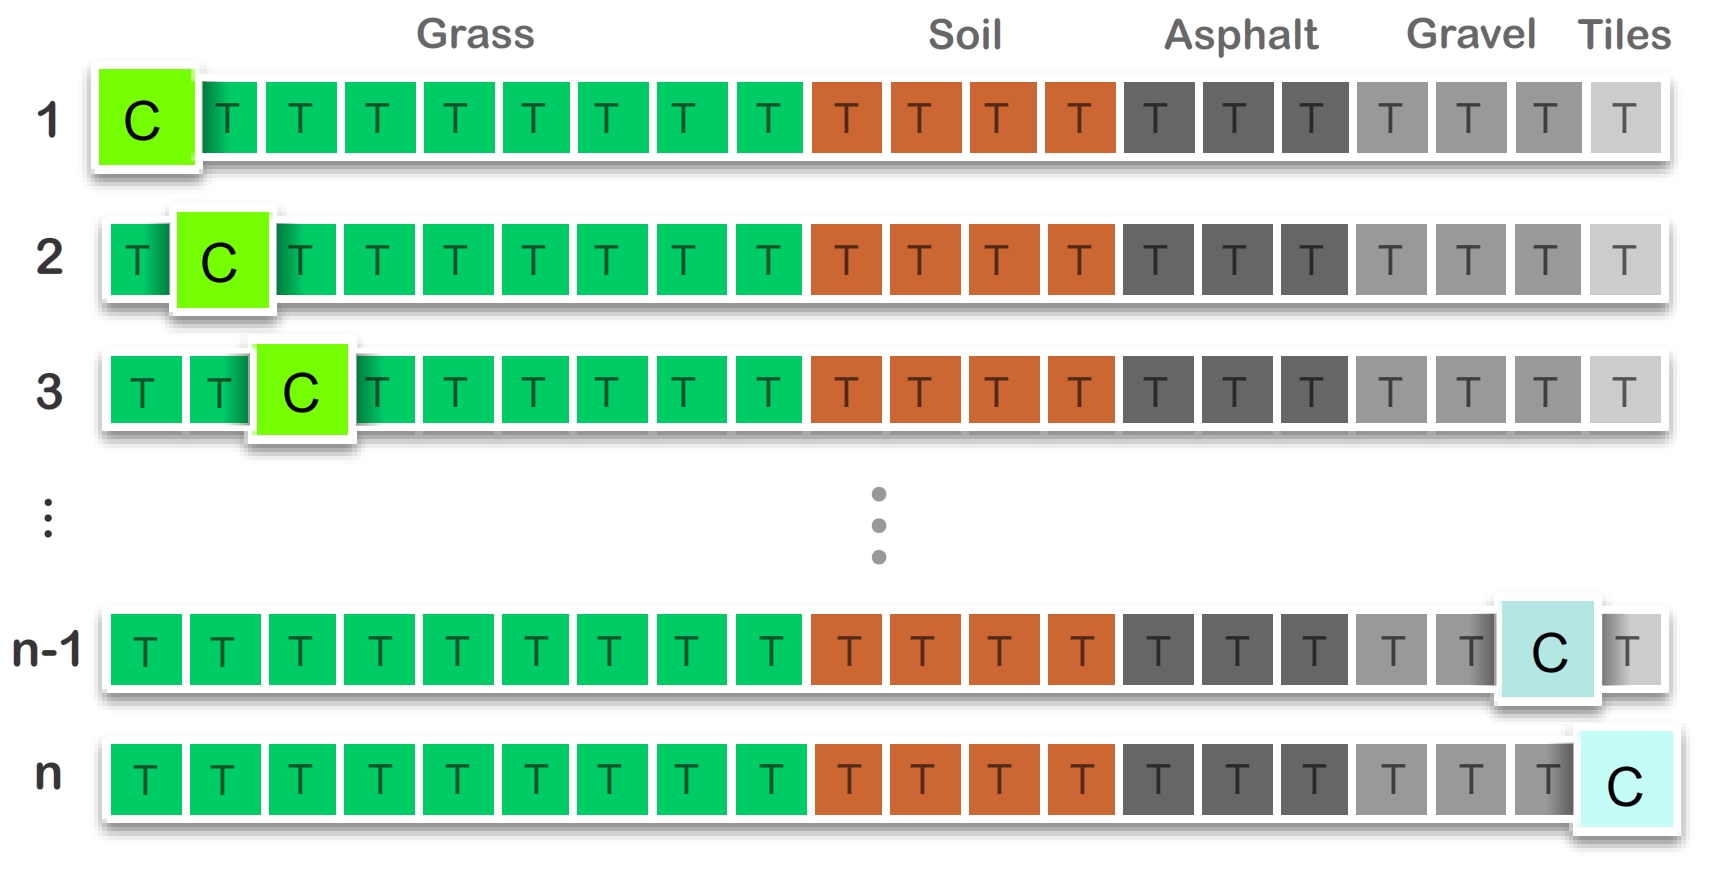
\includegraphics[scale=0.3]{figs_temp/loo.jpg}
	\caption{With the leave-one-out strategy, data is split up into $n$ parts. The model evaluation is done in $n$ steps - each time, one part of the data is excluded from the training and evaluated upon. The T's in the figure mark which parts of the data that are used for training, and the C's show what is used for classification.}
\end{figure}

%\rowcolors{2}{gray!25}{white}
\begin{table}
	\rowcolors{2}{gray!25}{white}
	\begin{center}
	\begin{adjustbox}{totalheight=\textheight-2\baselineskip}
		\begin{tabular}{|l|l|l|l|l|l|l|}
		\hline
		\rowcolor{gray!150}
		\rule{0pt}{25pt}\color{white}\textbf{Material} & \color{white}\textbf{LR} & \color{white}\textbf{RF} & \color{white}\textbf{\shortstack{LSTM\\CNN}} & \color{white}\textbf{SVM} & \color{white}\textbf{LDA} & \color{white}\textbf{DNN}\\
		Grass 1 & 97.9 & 98.05 & \cellcolor{red!20}59.0 & 95.75 & 96.8 & 97.45\\
		Grass 2 & 99.8 & 99.5 & \cellcolor{red!20}83.8 & 96.2 & 100.0 & 99.95\\
		Grass 3 & 94.35 & \cellcolor{red!20}86.75 & 94.5 & 91.4 & 92.6 & 95.3\\
		Grass 4 & 95.7 & 96.45 & 100.0 & 91.35 & 93.65 & 97.8\\
		Grass 5 & 96.65 & 97.25 & 97.4 & 93.95 & 95.9 & 95.55\\
		Grass 6 & 96.35 & 98.8 & 95.9 & 92.95 & 97.2 & 99.3\\
		Grass 7 & 99.9 & 99.85 & 99.9 & 99.65 & 99.95 & 100.0\\
		Grass 8 & 97.0 & 96.65 & 97.5 & 96.85 & 92.7 & 96.95\\
		Grass 9 & 97.75 & 97.7 & 99.8 & 97.8 & 96.3 & 98.75\\
		Grass 10 & 99.2 & 98.65 & 99.9 & 99.0 & 97.65 & 99.7\\
		Grass 11 & 99.35 & 98.7 & 99.9 & 99.25 & 97.55 & 99.8\\
		Grass 12 & 99.6 & 99.4 & 99.9 & 99.6 & 99.2 & 99.65\\
		Grass 13 & 100.0 & 100.0 & 100.0 & 100.0 & 99.85 & 100.0\\
		Grass 14 & 96.35 & 96.8 & 98.6 & 95.6 & \cellcolor{red!20}89.85 & 98.1\\
		Grass 15 & 97.6 & 95.45 & 99.8 & 93.1 & \cellcolor{red!20}87.4 & 99.05\\
		Grass 16 & 97.55 & 98.0 & 99.8 & 95.8 & 94.05 & 98.85\\
		Grass 17 & 95.4 & 92.85 & 98.4 & 94.6 & \cellcolor{red!20}89.9 & 95.0\\
		Grass 18 & 97.35 & 94.4 & 96.9 & 96.55 & 93.65 & 95.6\\
		\hline
		Asphalt 1 & 100.0 & 100.0 & 99.9 & 100.0 & 100.0 & 100.0\\
		Asphalt 2 & 99.95 & 100.0 & 99.0 & 100.0 & 100.0 & 100.0\\
		Asphalt 3 & 100.0 & 100.0 & 99.7 & 100.0 & 99.95 & 99.2\\
		Asphalt 4 & 99.9 & 99.85 & 100.0 & 99.9 & 99.95 & 100.0\\
		Asphalt 5 & 100.0 & 100.0 & 100.0 & 100.0 & 100.0 & 100.0\\
		Asphalt 6 & 100.0 & 100.0 & 100.0 & 100.0 & 99.9 & 99.95\\
		\hline
		Gravel 1 & 99.45 & 99.85 & 99.8 & 99.9 & 99.2 & 99.7\\
		Gravel 2 & \cellcolor{red!20}82.65 & 97.1 & \cellcolor{red!20}86.6 & \cellcolor{red!20}88.2 & \cellcolor{red!20}89.3 & 94.3\\
		Gravel 3 & 99.95 & 99.55 & 100.0 & 100.0 & 99.95 & 99.75\\
		Gravel 4 & 98.95 & 99.6 & 99.9 & 99.55 & 99.9 & 99.8\\
		Gravel 5 & 99.85 & 99.8 & 99.9 & 99.95 & 100.0 & 99.7\\
		Gravel 6 & 99.75 & 99.7 & 100.0 & 99.75 & 99.9 & 99.55\\
		\hline
		Soil 1 & 99.85 & 100.0 & 99.7 & 99.95 & 99.7 & 99.9\\
		Soil 2& 99.35 & 99.6 & 99.4 & 99.85 & 99.4 & 99.75\\
		Soil 3 & 99.75 & 99.85 & 100.0 & 100.0 & 99.9 & 99.85\\
		Soil 4 & 97.8 & 96.3 & \cellcolor{red!20}88.9 & 98.9 & 97.4 & 95.95\\
		Soil 5 & 96.25 & 95.45 & 100.0 & 96.55 & 96.55 & 93.95\\
		Soil 6 & 96.35 & 94.0 & 99.3 & 96.85 & 95.5 & 99.85\\
		Soil 7 & 92.65 & 95.15 & 99.3 & 90.25 & 92.4 & 100.0\\
		Soil 8 & 94.75 & 95.65 & \cellcolor{red!20}84.7 & 90.95 & 92.9 & 95.15\\
		\hline
		Tiles 1 & 99.35 & 99.4 & 100.0 & 99.55 & 99.3 & 99.35\\
		Tiles 2 & 99.95 & 99.75 & 99.9 & 99.95 & 99.6 & 99.95\\
		Tiles 3 & 99.95 & 99.9 & 100.0 & 100.0 & 100.0 & 99.95\\
		Tiles 4 & 99.95 & 99.7 & 99.5 & 99.95 & 100.0 & 94.45\\
		\hline
		\textbf{Mean} & 97.96 & 97.99 & 97.06 & 97.37 & 97.02 & \cellcolor{green!20}98.5\\
		\textbf{Median} & 99.35 & 99.4 & \cellcolor{green!20}99.8 & 99.4 & 99.2 & 99.68\\
		\textbf{SD} & 3.05 & 2.63 & 7.23 & 3.3 & 3.58 & \cellcolor{green!20}1.96\\
		\hline
		\end{tabular}
	\end{adjustbox}
	\end{center}
	\caption{Leave-one-out accuracies for all collected data series and the different models.}
	\label{tab:loo}
\end{table}

\subsection{Selecting a Model}
% I suggest removing this
%Optimizing each model presented above would of course be ideal, but also require much time and effort. Hence, we select what we regard as the most promising model based on the result of the leave-one-out evaluation. This model will then be optimized and more thoroughly evaluated.

Table \ref{tab:loo} shows the leave-one-out accuracies for all considered models. From the table we can see that all models perform well on every asphalt and tiled surface. Gravel, soil and grass are occasionally harder to classify correctly. Looking back at the principal component analysis in figure 4.4 this should not come as a great surprise as these are the main surface types with significant overlap. As for gravel, there is one measurement in particular that sticks out - Gravel 2. The accuracy of this is well below the average accuracy regardless of models. This could be beacuase this particular gravel contained characteristics not captured by the other gravel surfaces, resulting in several misclassifications. It also possible that some temporary problem occured in the measurement setup.

Another quirk worth noting is the great accuracy span of the \gls{lstm}-\gls{cnn} method. While it has a leading median score of 99.8 \%, it also contains several surfaces where it performed very poorly. This gives it the highest standard deviation among all the methods, suggesting it is not as robust as its competitors. It is possible that this could be remedied with a little bit of fine-tuning, but due to a limited amount of time, we disregard this model, making the  \gls{dnn}-model becomes the top performer with the greatest median and mean as well as the lowest standard deviation of the rest. Thus, for the remainder of this report, the \gls{dnn} model is used.







